\chapter{Results \& discussion} \label{chapter:interviews}

It should not be surprising that neither data scientists nor software engineers can be replaced by software libraries. However, a non-negligible subset of their processes can be partially or fully automated, especially when it comes to packaging and deploying AI/ML services. The objective was to design a library with an API that finds the balance between being simple enough to adopt without friction yet useful enough to be adopted. Simplicity is subjective and will be discussed separately in Section \ref{section:interviews}. For now, let us look at the utility of \textit{GreatAI}.

\section{Features} \label{section:features}

For answering \textbf{RQ3} --- \textit{To what extent can \textit{GreatAI} automatically implement AI deployment best practices?} --- a comparison is presented in the following, demonstrating a subset of best practices that can be implemented/scaffolded/configured with little user input; hence, through a simple and streamlined API. Tables \ref{table:best-practices-1} and \ref{table:best-practices-2} summarise the implemented best practices in the context of methods found by prior surveys of scientific and grey literature \cite{serban2020adoption,serban2021practices,john2020architecting}.

In order to show an accurately nuanced representation, a \textit{Level of support} is determined for each best practice on a scale of \textit{Partially supported}, \textit{Supported}, and \textit{Fully automated}. For instance, \textit{Use static analysis to check code quality} from Table \ref{table:best-practices-1} is \textit{Supported} because the entire public interface of \textit{GreatAI} is correctly typed (including generics and asynchronous coroutines) and compatible with \href{https://mypy.readthedocs.io/en/stable/index.html#}{\texttt{mypy}} and \href{https://marketplace.visualstudio.com/items?itemName=ms-python.vscode-pylance}{\texttt{Pylance}}. This means that when \textit{GreatAI} is used in any Python project, various tools can be applied to statically check the soundness of the project's integration with \textit{GreatAI}. However, if the library's user does not use type hints in their code and it contains a more complex control flow, it can only be partially type-checked. In short, this best practice is supported, and a considerable part of it is already implemented by \textit{GreatAI}, but clients should still keep in mind that they might also need to make an effort to implement it fully.

This is not the case for \textit{Log production predictions with the model's version and input data} because, by default, it is automatically implemented when calling \texttt{@GreatAI.create}. Users can still specify the exact expected behaviour, e.g., where to store traces, additional metrics to log, or disabling the logging of sensitive input. Nevertheless, the best practice is already implemented reasonably well without input from the library's user.

\begin{table}
\centering
\begin{threeparttable}
\caption{A subset of AI lifecycle best practices and the level of support \textit{GreatAI} provides for them. The level of support is one of \textit{Fully automated} (\checkmark\checkmark), which means that no action is required from the user, \textit{Supported} (\checkmark) only automates the reasonably automatable aspects, while \textit{Partially supported} ($\sim$) provides some useful features, but the client is expected to build on top of these.}

\label{table:best-practices-1}
{\renewcommand{\arraystretch}{1.2} % for the vertical padding
\begin{tabular}{P{7cm}@{\hskip 0.5cm}l@{\hskip 0cm}c} \hline

\textbf{Best practice}                                                                    & \textbf{Implementation}                        & \textbf{Support}       \\\hline
Use sanity checks for all external data sources\textsuperscript{1}                        & \texttt{@parameter}                            & \checkmark             \\\hline
Check that input data is complete, balanced, and well-distributed\textsuperscript{1}      & \texttt{@parameter}                            & $\sim$                 \\\hline
Write reusable scripts for data cleaning and merging (for NLP)\textsuperscript{1}         & \texttt{utilities}                             & \checkmark\checkmark   \\\hline
Make datasets available on shared infrastructure\textsuperscript{1}                      & \texttt{large\_file}                           & \checkmark\checkmark   \\\hline
Test all feature extraction code (for NLP)\textsuperscript{1}                             & \texttt{utilities}                             & \checkmark\checkmark   \\\hline
Employ interpretable models when possible\textsuperscript{1}                              & \texttt{views}                                 & $\sim$                 \\\hline
Continuously measure model quality and performance\textsuperscript{1, 2}                  & Feedback API                                   & \checkmark             \\\hline
Use versioning for data, model, configurations and training scripts\textsuperscript{1, 2} & \texttt{@use\_model}, versioning               & \checkmark\checkmark   \\\hline
Run automated regression tests\textsuperscript{1}                                         & \texttt{*\_ground\_truth}                      & \checkmark             \\\hline
Use continuous integration\textsuperscript{1}                                             & Docker Image, WSGI application                 & \checkmark             \\\hline
Use static analysis to check code quality\textsuperscript{1}                              & Fully typed API with generics                  & \checkmark             \\\hline
Assure application security\textsuperscript{1}                                            & Code is automatically audited                  & $\sim$                 \\\hline
Automate model deployment, enable shadow deployment\textsuperscript{1, 2}                 & Docker Image \& scripts                        & \checkmark             \\\hline
Enable automatic rollbacks for production models\textsuperscript{1, 2}                    & Docker Image \& scripts                        & $\sim$                 \\\hline
Continuously monitor the behaviour of deployed models\textsuperscript{1, 2}               & Dashboard, metrics endpoints                   & \checkmark\checkmark   \\\hline
Log production predictions with the model's version and input data\textsuperscript{1}     & \texttt{@GreatAI.create}                       & \checkmark\checkmark   \\\hline

\end{tabular}}
\begin{tablenotes}
    \item[1] SE4ML best practices from Table 2 of \cite{serban2020adoption}, and Table 1 of \cite{serban2021practices}.
    \item[2] Reported state-of-the-art and state-of-practice practices from Tables 2, 3, and 4 of \cite{john2020architecting}.
\end{tablenotes}
\end{threeparttable}
\end{table}

\begin{table}
\centering
\begin{threeparttable}
\caption{A subset of AI lifecycle best practices and the level of support \textit{GreatAI} provides for them. The level of support is one of \textit{Fully automated} (\checkmark\checkmark), which means that no action is required from the user, \textit{Supported} ($\checkmark$) only automates the reasonably automatable aspects, while \textit{Partially supported} ($\sim$) provides some useful features but the client is expected to build on top of these.}

\label{table:best-practices-2}
{\renewcommand{\arraystretch}{1.2} % for the vertical padding
\begin{tabular}{P{7cm}@{\hskip 0.5cm}l@{\hskip 0cm}c} \hline

\textbf{Best practice}                                                                    & \textbf{Implementation}                        & \textbf{Support}       \\\hline
Execute validation techniques: error rates and cross-validation\textsuperscript{2}        & \texttt{*\_ground\_truth}                      & \checkmark             \\\hline
% Track models, dependencies, experiments, versions\textsuperscript{2}                    & \texttt{great\_ai.use\_model}, Dashboard       & \checkmark\checkmark   \\\hline
Store models in a single format for ease of use\textsuperscript{2}                        & \texttt{save\_model}                           & \checkmark\checkmark   \\\hline
Rewrite from data analysis to industrial development language\textsuperscript{2}          & Jupyter Notebook deployment                    & \checkmark             \\\hline
Equip with web interface, package image, provide REST API\textsuperscript{2}              & \texttt{@GreatAI.create}                       & \checkmark\checkmark   \\\hline
Provide simple API for serving batch and real-time requests\textsuperscript{2}             & \texttt{@GreatAI.create}                       & \checkmark\checkmark   \\\hline
For reproducibility, use standard runtime and configuration files\textsuperscript{2}      & \texttt{utilities.ConfigFile}, Dockerfile      & \checkmark             \\\hline
Integration with existing data infrastructure\textsuperscript{2}                          & GridFS, S3 support                             & \checkmark\checkmark   \\\hline
Select ML solution fully integrated with databases\textsuperscript{2}                     & MongoDB, PostgreSQL support                    & \checkmark\checkmark   \\\hline
Querying, visualising and understanding metrics and event logging\textsuperscript{2}      & Dashboard, Traces API                          & \checkmark\checkmark   \\\hline
% Monitor status and performance\textsuperscript{1, 2}                                    & Dashboard, Status (metadata) API               & \checkmark\checkmark   \\\hline
Measure accuracy of deployed model to ensure data drifts are noticed\textsuperscript{2}   & Feedback API                                   & \checkmark             \\\hline
Apply automation to trigger model retraining\textsuperscript{2}                           & Feedback API                                   & $\sim$                 \\\hline
% Employ Agile, DevOps-style workflows, allow automatic rollback\textsuperscript{2}       & Docker Image, WSGI application                 & \checkmark             \\\hline
% Deploy different versions of same application\textsuperscript{2}                        & Complex versioning support                     & $\sim$                 \\\hline
Allow experimentation with the inference code\textsuperscript{3}                          & Development mode \& auto-reload                & \checkmark\checkmark   \\\hline
Keep the model's API and documentation together\textsuperscript{3}                        & Dashboard and Swagger                          & \checkmark\checkmark   \\\hline
Parallelise feature extraction\textsuperscript{3}                                         & \texttt{parallel\_map}                         & \checkmark\checkmark   \\\hline
Cache predictions\textsuperscript{3}                                                      & \texttt{@GreatAI.create}                       & \checkmark\checkmark   \\\hline
Support asynchronous top-down chaining of models\textsuperscript{3}                       & All decorators support async                   & \checkmark\checkmark   \\\hline
Implement standard schemas for common prediction tasks\textsuperscript{3}                 & \texttt{views}                                 & \checkmark             \\\hline

\end{tabular}}
\begin{tablenotes}
    \item[2] Reported state-of-the-art and state-of-practice practices from Tables 2, 3, and 4 of \cite{john2020architecting}.
    \item[3] Additional software engineering best practices applicable to AI/ML deployments encountered while designing and using \textit{GreatAI}.
\end{tablenotes}
\end{threeparttable}
\end{table}

\FloatBarrier

In Table \ref{table:best-practices-2}, we added six additional best practices, which are generally well-known software engineering considerations that are also applicable to AI/ML deployments. These had not explicitly made it into the aforementioned surveys; however, according to the insights gained from Sections \ref{section:simple-case} and \ref{section:complex-case}, implementing them has a positive effect on deployment quality. In future research, attention could be given to their level of industry-wide adoption and quantitative utility.

Quantifying the number of implemented best practices would be misleading since their scope and importance cover a wide range; furthermore, there is some overlap between the different studies and even within the studies. However, it is still clear that a large number of best practices (17) can be given a \textit{Fully automated} implementation by \textit{GreatAI}'s design, and many others (16) can be augmented by the library. This proves the feasibility of designing simple APIs using the techniques of Chapter \ref{chapter:design} for decreasing the complexity of correctly deploying AI services while still implementing various best practices (\textbf{RQ2}).

\section{Interviews} \label{section:interviews}

One of the central takeaways of Section \ref{section:existing} is that, for example, Seldon Core is useful for implementing or helping to implement most of the best practices. Regardless, it also has an initial threshold that must be surmounted before implementing even a single one. According to the adoption rate surveys, this may discourage a large portion of practitioners from using it or other similar frameworks. The presented solution offers a different mix of features: the initial threshold is virtually non-existent; hence, best practices can be applied immediately. But at the same time, it only covers a more limited range of practices. 

Our hypothesis is that the latter approach aligns better with the expectations of professionals. To verify this, we conducted a series of interviews with the cooperation of ten industry practitioners with varying levels of Software Engineering (SE) and Data Science (DS) experience. In this section, the question of generalisability (\textbf{RQ4}) is investigated using the interview methodology described in Section \ref{section:interview-setup}. The participants were gathered through the recommendations of my friends and colleagues. All of the final interviewees have had at least some expertise in both DS (with a median of 2.5 years) and SE (with a median of 2 years).

\subsection{Best practices survey} \label{subsection:best-practices-survey-results}

The practitioners were first asked to fill out a questionnaire about their latest AI/ML project involving deployment. This point-in-time measurement (shown in Appendix \ref{appendix:practices}) served as a baseline for the deployment quality they are used to. Analysing the results show that the amount of software engineering experience has a moderately strong correlation ($r_{Pearson} = 0.67$ with $p = 0.0033$) with the overall number and extent of implemented deployment best practices. This is illustrated in Figure \ref{fig:adoption}. Interestingly but unsurprisingly, there is no similar statistically significant relationship regarding the amount of data science experience. 

The y-axis of Figure \ref{fig:adoption} is calculated by discarding the \textit{Not applicable} answers and projecting the 5-point Likert scale to a range from 0 to 1, which is subsequently averaged over all questions. The overall mean adoption rate/extent is just above 0.5, which equates to the \textit{Neither agree nor disagree} label. These data are in line with the findings of Serban et al. \cite{serban2020adoption}.

Because the survey's 15 questions were compiled from the \textit{Fully automated} rows of Tables \ref{table:best-practices-1} and \ref{table:best-practices-2}, that means that when using \textit{GreatAI}, they are all implemented automatically. Consequently, the adoption rate/extent is doubled immediately just by wrapping the inference function with \texttt{@GreatAI.create}: this is the added value of \textit{GreatAI}\footnote{As explained earlier, measuring quality as a function of best practice count would be dubious. Thus, the achieved magnitude of the doubling is irrelevant; however, the direction of change is not.}. Moreover, this provides further evidence for answering \textbf{RQ3} showing the extent of automatically implemented practices over non-\textit{GreatAI} deployments.

\begin{figure}
    \centering
    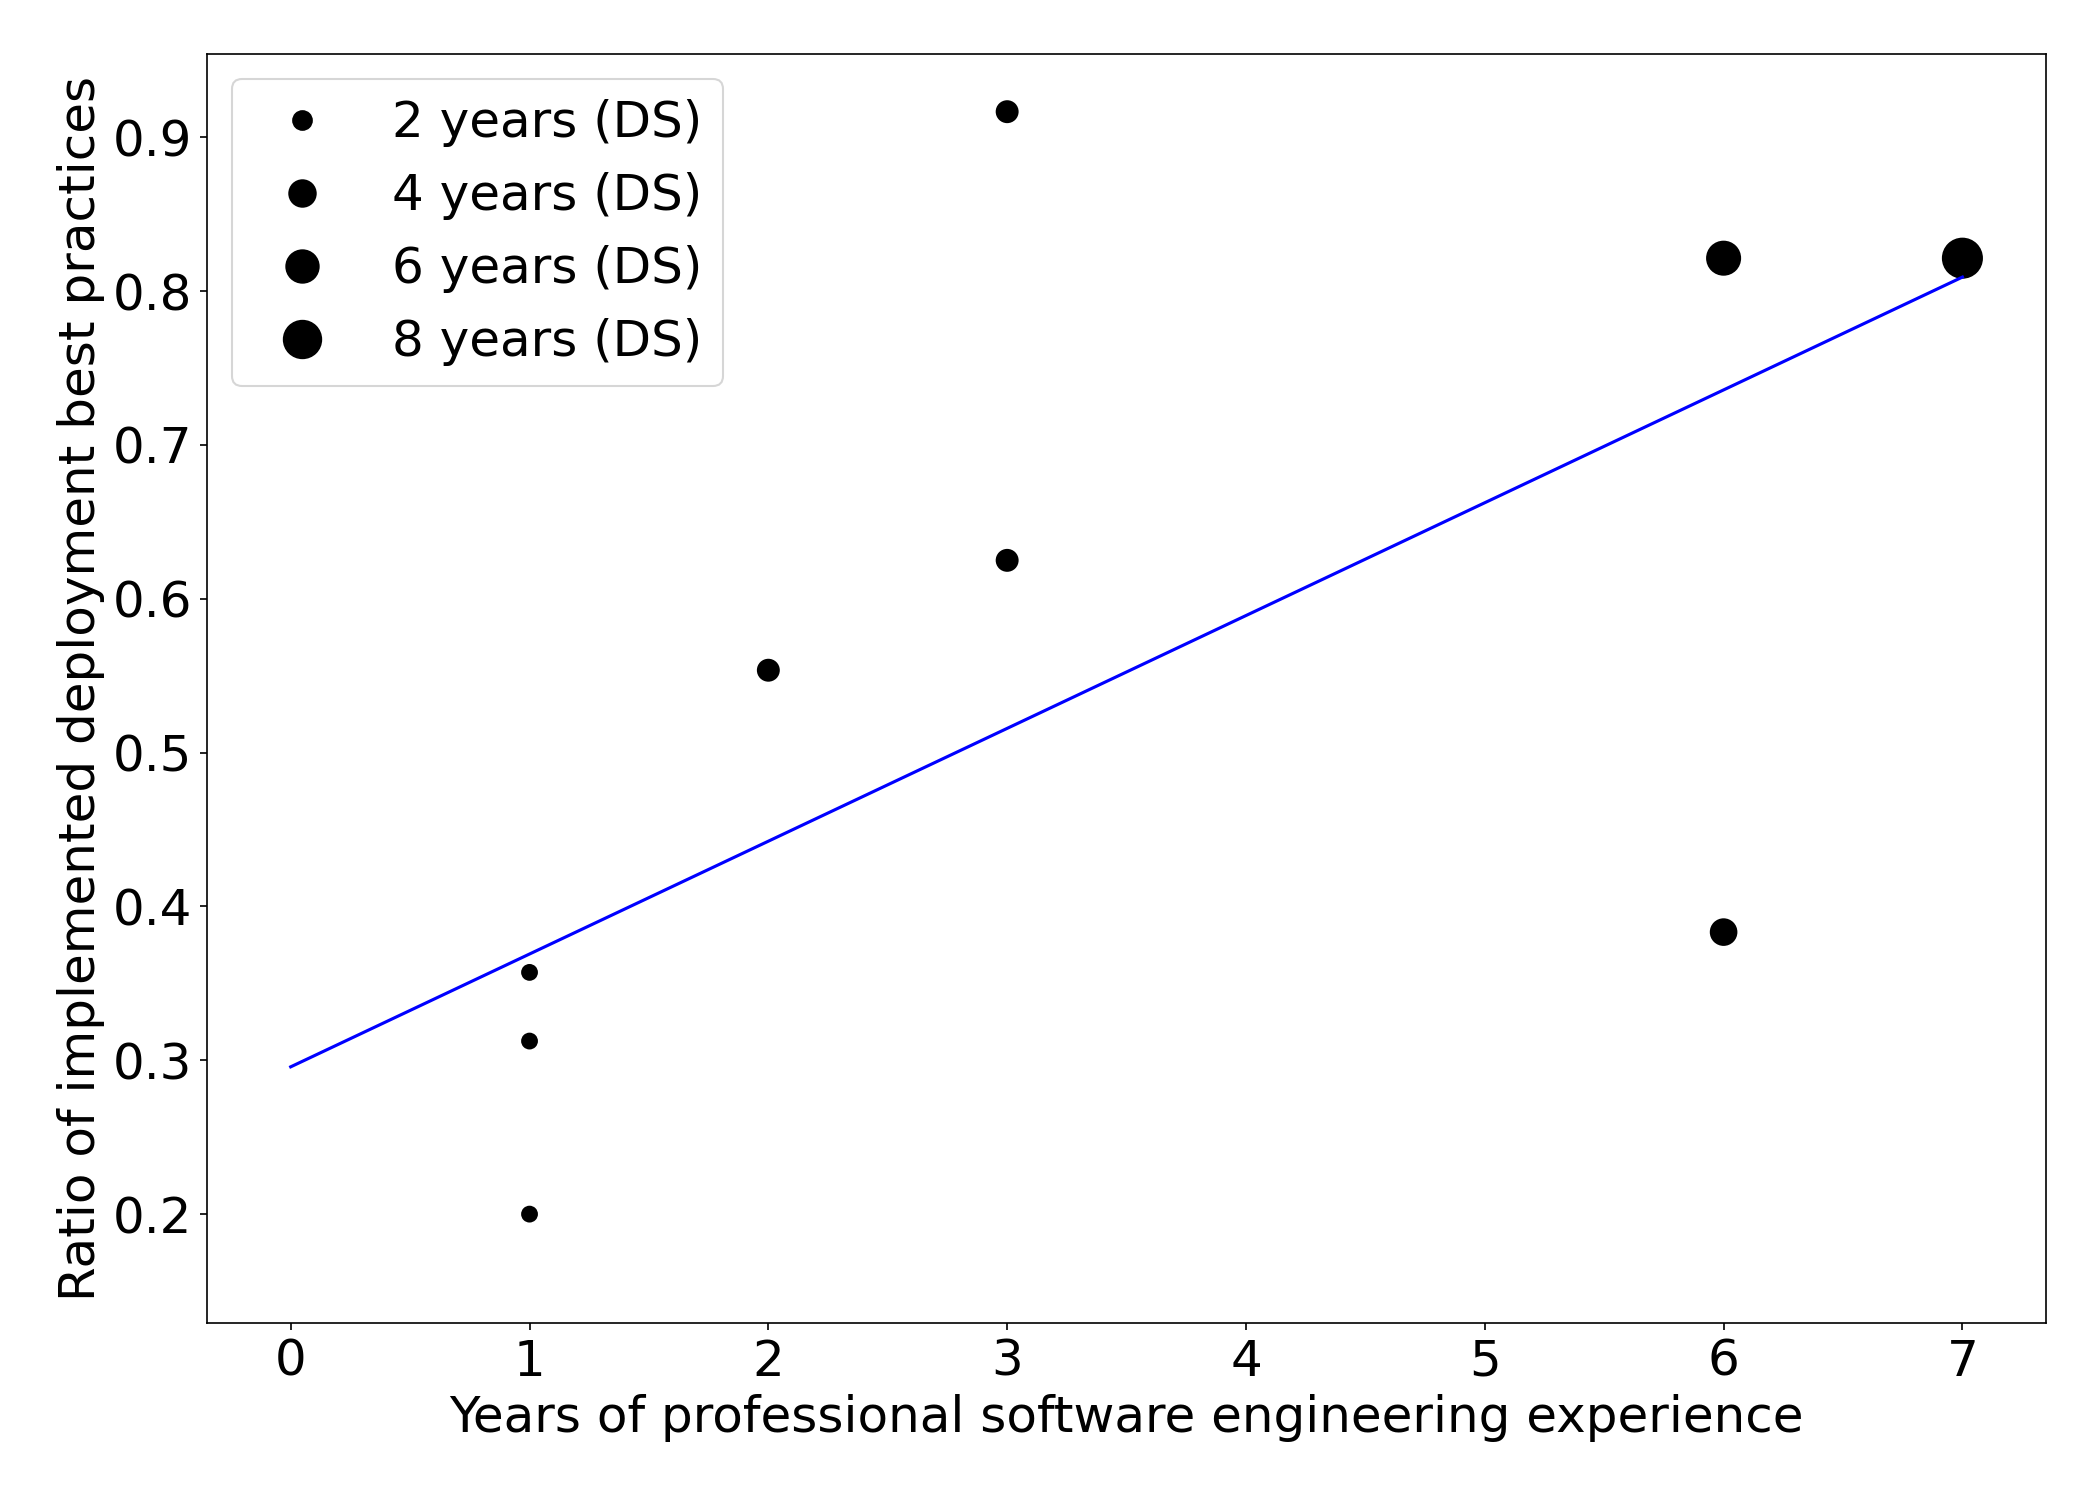
\includegraphics[width=0.6\linewidth]{figures/best-practices.png}
    \captionsetup{width=.9\linewidth}
    \caption{Best practices adoption rate as a function of Software Engineering (SE) and Data Science (DS) experience. SE experience is shown on the horizontal axis, while the point sizes denote the practitioners' experience in DS. The correlation between the axes is significant ($r_{Pearson} = 0.67$ with $p = 0.0033$).}
    \label{fig:adoption}
\end{figure}

\subsection{Technology acceptance}

\begin{table}[H]
\centering
\captionsetup{width=.9\linewidth}
\caption{Technology acceptance model survey (presented in Appendix \ref{appendix:questions}, sample size = 10) results per variable. The input values range from 1 to 7.}
\label{table:tam}
{\renewcommand{\arraystretch}{1.1} % for the vertical padding
\begin{tabular}{|r|l|l|l|} \hline
                            & \textbf{Perceived ease of use} & \textbf{Perceived utility} & \textbf{Intention to use} \\\hline
\textbf{Median}             & 5.8                          & 6.4                      & 6.3                     \\\hline
\textbf{Mean}               & 5.5                          & 6.1                      & 6.0                     \\\hline
\textbf{Standard deviation} & 1.0                          & 0.9                      & 1.3                     \\\hline
\textbf{Cronbach's alpha}   & 0.77                         & 0.88                     & 0.95                     \\\hline
\end{tabular}}
\end{table}

The participants filled out a form (shown in Appendix \ref{appendix:questions}) after finishing their first deployment with \textit{GreatAI} to provide data for creating the technology acceptance model of the problem context. The survey contained ten questions from three categories, which could be rated on a 7-point Likert scale. The summary of the answers is presented in Table \ref{table:tam}. The high Cronbach's alpha values indicate strong internal consistency \cite{nunnally1994psychometric} for each TAM dimension; thus, averaging the responses per category is semantically meaningful.

Following the methodology of \cite{cruz2019catalog}, the connections between the Perceived Utility (PU), Perceived Ease Of Use (PEOU), and Intention To Use (ITU) dimensions of TAM were analysed. Two statistically significant ($P \leq 0.05$) correlations were uncovered: between PU and ITU ($r_{Pearson} = 0.81$ with $p = 0.0048$); and PEOU and ITU ($r_{Pearson} = 0.80$ with $p = 0.0068$). Learning from the findings of prior case studies, it is reasonable to believe that both the \textit{perceived utility} and the \textit{perceived ease of use} play an equally important role in influencing professionals' \textit{intention to use} the deployment framework.

The assessment of \textit{ease of use} lags behind the rest, but it is still quite high. It may be possible that PEOU would go up with further use. Nevertheless, the high \textit{perceived utility} implies that \textit{GreatAI} shows its value early on. This, combined with the correlations uncovered within the context's technology acceptance model, validates the hypothesis that focusing on good API design is just as necessary as providing practical features.

\subsection{Task solving \& exit interviews}

In order to give qualitative depth to the previously presented quantitative results, it is time to discuss the main segment of the interviews. The participants' backgrounds covered a vast and fascinating cross-section of industrial AI/ML. The financial sector was represented by a researcher working on market prediction models for the Hungarian State Treasury and two people building an upcoming digital bank's core services. Image processing contexts were illustrated by professionals predicting Sun activity at the European Space Agency and different ones creating pose-recognition at a startup for people with disabilities using 3D cameras. Moreover, investigating companies' AI use as part of due diligence processes and intrusion detection from network packet traces are just some of the other core activities the interviewees had been doing recently. 

Stemming from this diversity, these semi-structured interviews could be expected to provide valuable insights into the generalisability of \textit{GreatAI}. The methodology of Section \ref{section:interview-setup} was followed by applying reflective journaling and thematic analysis. After labelling each aspect of the feedback, and two iterations of merging redundant or related topics, we ended up with three overarching themes: \textit{Functionality}, \textit{API}, and \textit{Responsibility to adopt}. As we will soon see, these correspond to the \textit{perceived utility}, \textit{perceived ease of use}, and \textit{intention to use} components of TAM fairly well.

\paragraph{Functionality} The library's feature-set was complimented during most interviews, with one participant noting that, although the overall number of features is relatively small, most of them are utilised in most cases. Similarly, the \texttt{utilities} submodule was appreciated for helping greatly in the interview task, but non-NLP researchers noted its likely inadequacy for their area. Still, they would like to see ``bundle'' or ``toolbox''-style modules for their fields because it would save them from a lot of copy-pasting.

The effortless parallel feature extraction and large file handling support were highlighted multiple times for the reason that the particular interviewees had not encountered other libraries providing these features. Other concrete features, such as the searchable \textit{exceptions} column in the Dashboard's table and the \textit{feedback} mechanism, were also popular. One professional highlighted the latter for coercing users to consider a human-in-the-loop approach which was said to be often expected in modern systems.

When reflecting on the framework from a bird's eye view, the generality and extensibility of the API were emphasised. As explained by a senior engineer, this is mainly because once you commit to using it, it is important not to find yourself at a dead end for a specific use case forcing you to look for a different library. However, two participants also noted that for complete generality, \texttt{MATLAB} support would be necessary. Regarding non-functional features, private hosting (especially in banking and government), open-source auditability, and good scalability (by means of an external database) were the top subjects of praise.

\paragraph{API} Regarding the surface through which clients interact with the library, the feedback is also positive but more nuanced. Many participants liked that the functions' behaviour is easy to guess from their names. The decorator syntax caused minor confusion but consulting the documentation solved the issues in all three cases. The CLI app \texttt{great-ai} was appreciated for having a close to trivial signature; the participant noted that she strives to use as few CLI commands as feasible. Surprisingly, even the practitioners with more data science background appreciated the Docker support. Nonetheless, one expert had a feature request for a configuration GUI because his colleagues are used to handling MATLAB App Designer applications.

The recurring theme of the discussions focused on the question of ``\textit{How simple is too simple?}''. The argument is that an API cannot be simpler than the domain in which it exists. More precisely, it can only be simpler at the cost of losing transparency. Let us take the example of saving models using \texttt{save\_model()}. If a project is set up correctly, it either has an initial \texttt{configure()} call to the storage provider backend, or it has an appropriately named credentials file in the project's root, for instance, \texttt{s3.ini} or \texttt{mongo.ini}. Once set up, it is trivial to use as long as we do not divert from the happy path. However, if an issue arises, such as an upgrade or migration of MongoDB, debugging the application is non-trivial for its lack of transparency.

In other words, we could say that the average (cognitive) complexity is low while the worst-case is as high --- if not higher --- than without using \texttt{save\_model()}. This proved to be somewhat controversial. However, ultimately, optimising the happy path of the AI/ML development lifecycle was deemed worthwhile by the participants in most cases. With the argument that the majority of the time spent during a project is spent on this path anyway. However, this raises the question of who exactly are the target users of \textit{GreatAI} and who will fix arising issues?

\paragraph{Responsibility to adopt} Let us first look at some insightful anecdotes that surfaced during the interviews. Especially in more research-oriented environments, production deployment pipelines can be of questionable robustness. This phenomenon was demonstrated by one account of a simple single-machine deployment pipeline: it is an interplay of \texttt{cron} jobs calling a series of shell and MATLAB scripts resembling a Rube Goldberg machine. But connecting a couple of Google Colab accounts to a GitHub repository and Weights\&Biases\footnote{\href{https://wandb.ai/site}{wandb.ai}} to implement parallel model training can also be found in the wild.

Moreover, various research companies were mentioned that for multiple years used to or still have an R\&D department consisting solely of data scientists. In one extreme case, the staff was described as more than 30 data scientists and 0 other technical employees. In such a setup, it is unreasonable to expect even professionals to have the capabilities and focus to set up the required foundation for handling all best practices. All but one interviewee verified this assumption. They also referred to their previous projects, which usually required many researchers and experts from various fields, and too often, software engineers had not been prioritised to be included.

Doing software engineering without software engineers is difficult. \textit{GreatAI} is not a viable replacement for any well-trained expert, though it is still better than nothing. During the interviews, we realised that the likely underlying reason for not employing AI engineers or software engineers as part of AI/ML projects is a lack of awareness. This was theorised by some and demonstrated by six participants who had, even though followed some, not explicitly sought out information on AI deployment best practices. Thus, raising awareness --- especially by presenting a value proposition, e.g. lower maintenance costs and better long-term quality --- might be crucial for improving AI deployments in general. Verifying this hypothesis could be a worthwhile direction for future research.

During the larger discussions, \textit{GreatAI} was deemed appropriate for raising awareness since it showcases how even a simple library is able to implement a lot of best practices. Additionally, it was noted that it could also be considered for one-person projects where --- by definition --- it is admissible to have no SE expert on the ``team''. To further help such cases, integrating a one-click Heroku\footnote{\href{https://www.heroku.com/}{heroku.com}} app deployment was also recommended to simplify the entire last portion of the lifecycle. 

\subsection{Discussion of interviews}

The overall takeaway from this is that most features were well-received, and the high mean value of \textit{perceived utility} is credible. The criticism of being NLP-centric is also justified: the initial scope of the proof-of-principle framework was limited to this domain. Nonetheless, learning the experts' opinion that they wish to have a similarly specific solution to their problem contexts is reassuring because it proves that the API is not only generalisable but is expected to be generalised. At the same time, it is crucial to admit that no one-size-fits-all solution can exist for such a diverse domain. Therefore, allowing customisability and easy extension of the system must remain central design questions.

Regarding the API's level of abstraction, we have to agree with the experts that the problem of deployment cannot be ``magically'' solved by a trivial API. However, solving deployment problems can be streamlined, at least in simpler cases. At the same time, the complex ones can be left to the professionals with relevant knowledge. This parallels the AI-libraries that have inspired \textit{GreatAI}. For instance, Hugging Face \texttt{transformers} streamlines fine-tuning and applying SOTA models, but it does not provide any facilities to help you create the next SOTA architecture because that is a vastly more complex task that most users are not expected to tackle.

In order to reach its goal of improving best practice adoption, \textit{GreatAI} can help raise awareness by presenting a verifiable value proposition, i.e. a couple of lines of code can already result in more maintainable, robust, high-quality deployments. This might prompt users or technical decision-makers to invest more in software engineering in AI/ML projects. Additionally, it can help the effectiveness of AI/software engineers by handling the grunt work of implementing some best practices, leaving them with more resources to focus on the complex and creative aspects of \textit{GREAT} deployments.
  
In summary, the answer to \textit{How suitable is the design of GreatAI for helping to apply best practices in other contexts?} (\textbf{RQ4}) is --- unsurprisingly --- subjective. Combining the high value of \textit{intention to use} from Table \ref{table:tam}, the generally positive feedback regarding the library's added value, and the numerous feature requests for fitting it to specific needs, we conclude that there is some chance of suitability for generalisability. The existence of this potential is already exciting and presents an opportunity for experimenting with building on the design of \textit{GreatAI}.

\subsection{Threats to validity}

Two potential threats to the validity of the experiments and their results are identified. Firstly, the claimed utility of the framework derived in Subsection \ref{subsection:best-practices-survey-results} does not take into account the practical significance of the implemented features and, therefore, may be subject to bias. However, the \textit{perceived utility} evaluations indicate that the participating engineers and scientists identify practical value in the features of \textit{GreatAI}. Nevertheless, in the future, we intend to extend the range of implemented best practices, which would in turn, give higher confidence about the achievable quantitative improvement through using the library.

Secondly, the survey answers and, in general, the interviewees may be subject to bias. The small sample size of practitioners can reasonably lead to some groups being over- or under-represented. The presence of selection bias is also plausible. These could be mitigated by gathering more data in future research. Coming from the exploratory nature of this analysis, many insights could be gained from the collected data. However, for confidently generalising the results, more data are needed.

\section{Future work} 

The primary purpose of the library was to serve as a proxy through which its design decisions could be tested and evaluated in their practical context. For this reason, its design aimed to be a proof-of-principle for validating hypotheses and answering research questions. After successfully doing that, it has been turned into a practical software library suitable for production-use\footnote{Available at \href{https://pypi.org/project/great-ai/}{pypi.org/project/great-ai} and \href{https://hub.docker.com/repository/docker/schmelczera/great-ai}{hub.docker.com/repository/docker/schmelczera/great-ai}.}. 
 
The library's main limitations come from its bias toward NLP deployments. This is not unreasonable given the design's exploratory nature and the context of the case studies. Nevertheless, future work must focus on introducing and balancing support for many more fields' deployments. Although \textit{GreatAI} has already proved its utility, it has also shown that generalising and extending its functionality would be worthwhile. Therefore, many potential improvements are presented below.

\subsection{More ML fields}

The cases presented in Chapter \ref{chapter:case} revolved around NLP. This, of course, heavily influenced the design process. The two most notable effects can be found in the REST API's \texttt{/predict} endpoint and some \texttt{utilities} functions. The former is streamlined to accept JSON-compatible data (which caters to textual and tabular data), while the latter gives robust feature extraction support only for textual input. However, in practice, sound, image, and video are also widely taken as input. Furthermore, with the rise of multimodal models \cite{gao2020survey}, even different combinations of them may be simultaneously taken as input.

Supporting the easy, direct upload of larger non-JSON files --- e.g. by saving them to S3 and showing a preview of them on the Dashboard's traces table --- and extending \texttt{utilities} to handle multimedia formats should be sufficient for counteracting the NLP bias. Hence, widely expanding the scope of applicability of \textit{GreatAI}. As we have seen in Section \ref{section:architecture}, the architecture is otherwise adequately general; therefore, incremental extensions can be applied.

\subsection{More best practices}

In order to greatly simplify its API, each \textit{GreatAI} Trace is a single document with a well-defined schema that clients can also extend by calling \texttt{log\_metric}. MongoDB provides a convenient (and popular) method for persisting such documents; however, if there is some existing database in the environment, storing Traces in that can be favourable. PostgreSQL \cite{momjian2001postgresql} is a popular choice, and it also features good JSON document support. Hence, introducing first-class integration for PostgreSQL could benefit some clients.

Data-intensive services can fall into three broad categories: online systems, batch processing, and stream processing (near-teal-time systems) \cite{kleppmann2017designing}. As of yet, \textit{GreatAI} only provides streamlined support for the first two. Thus, developer experience could be improved by providing simple, direct integration with popular message queues/protocols, such as \href{https://kafka.apache.org/}{Apache Kafka} \cite{kreps2011kafka}, \href{https://aws.amazon.com/sqs/}{AWS SQS} \cite{garfinkel2007evaluation}, or \href{https://www.amqp.org/}{AMQP} \cite{vinoski2006advanced}. Moreover, some metrics of \textit{GreatAI}, such as the cache statistics, versions, and derived data from traces, can already be conveniently queried from its REST API. Nevertheless, adding support for the de facto standard metric gathering tool, Prometheus\footnote{\href{https://prometheus.io/}{prometheus.io}}, could save the library's users from one more integration step.

The common theme among the opportunities mentioned above is that they could be implemented reasonably well without any user input, which aligns with the library's philosophy. Of course, the open-source nature of \textit{GreatAI} already allows anyone to provide support for a wide range of integrations. Additionally, the scope could be reasonably extended, i.e. more practices could be incorporated by including more criteria next to the \textit{GREAT} ones.
